
%------------------------------------------------------------------------------------------------------
%  toto je zaklad prvej kapitoly, podstatna je zmena pagestyle na headings.
%  v chapter{} zadate meno prvej kapitoly, v label date nejake jednoduche oznacenie, 
%  idealne chap: na zaciatku, ako ze je to label pre kapitolu a potom nejaky slug pre konkretnu
%------------------------------------------------------------------------------------------------------
\chapter{Meno prvej kapitoly}\label{chap:prva}
\pagestyle{headings}

%------------------------------------------------------------------------------------------------------
%  Sem napiste nejaky text cisto v kapitole, este nie v podkapitole
%------------------------------------------------------------------------------------------------------
Tak tu date nejaky text v samotnej kapitole, nie este v podkapitole. Prepacte moje pisanie, len je uz doste vecer


%------------------------------------------------------------------------------------------------------
%  takto pridavajte podkapitoly/sekcie. zadate do zatvoriek nazov sekcie 
%  a za label do zatvoriek skratku pre tuto sekciu. To ak by ste sa chceli niekedy odkazovat
%------------------------------------------------------------------------------------------------------
\section{Meno sekcie/podkapitoly}\label{sec:firstoffirst}

Sem date text podkapitoly. Ako iste viete, novy odstavec sa dava tak 

ze date dva entery.

\section{Zakladne odrazky}

Cize teraz staci ukazat, ako pouzivat nejake zakladne odrazky. Vsak nie zakladne si mozete vyskusat samy.

%------------------------------------------------------------------------------------------------------
% Takto zacnete cast s vysvetleniami, kazdy item je nova polozka, ktora moze mat meno
%------------------------------------------------------------------------------------------------------
\begin{description}
	\item[Meno polozky] \hfill \\
Popis:
Lorem ipsum dolor sit amet, consectetur adipiscing elit. Maecenas convallis consectetur leo, sit amet feugiat diam consectetur ornare. 
Donec cursus nunc a quam convallis sit amet pretium ipsum elementum. Nam hendrerit felis a sapien facilisis egestas. 
Nunc non ultricies turpis. Suspendisse iaculis tempor neque, et lacinia erat pellentesque eu. Mauris aliquam dui id elit luctus molestie. 
Vestibulum ac metus elit. Aenean eget leo ligula. Ut aliquet congue justo, sed ultrices eros adipiscing vel. Cras hendrerit convallis arcu nec sodales. 
Etiam nisl lorem, auctor eu hendrerit vel, semper vel sapien. Morbi eu consectetur purus. Fusce dignissim dignissim ipsum ac tristique. 
Quisque sit amet augue eget nibh tincidunt lacinia. Nunc et dictum sapien.
\\Novy riadok date dvoma bakslashmi :)
%------------------------------------------------------------------------------------------------------
% Takto zacnete cast s odrazkami, kazdy item je nova polozka
%------------------------------------------------------------------------------------------------------
\begin{itemize}
	\item prihlásiť sa, optimálne by si mala aplikácia toto prihlásenie pamätať,
	\item vyhľadať svojho pokytovateľa a otvoriť správnu službu,
	\item ľahko sa orientovať v kalendári a nájsť potrebný termín,
	\item vytvoriť rezerváciu, v prípade, že používateľ nie je prihlásený, povoliť ju s požiadavkou základných údajov,
	\item zobraziť vlastné rezervácie,
	\item upraviť čas rezervácie podľa potreby,
	\item zrušiť rezerváciu,
	\item vytvoriť poskytovateľa.
\end{itemize}
%------------------------------------------------------------------------------------------------------
%  po tialto su gulickove odrazky
%------------------------------------------------------------------------------------------------------
	\item[Druhy pojem na vysvetlenie] \hfill \\
Ako vidite, daju sa vysvetlenia a odrazky vnarat. Mozete sa pohrat ako chcete :)
\end{description}

Este zostava ako pridat nejaky obrazok, cize tu je ukazka

\begin{figure}[h]
	\centering	
		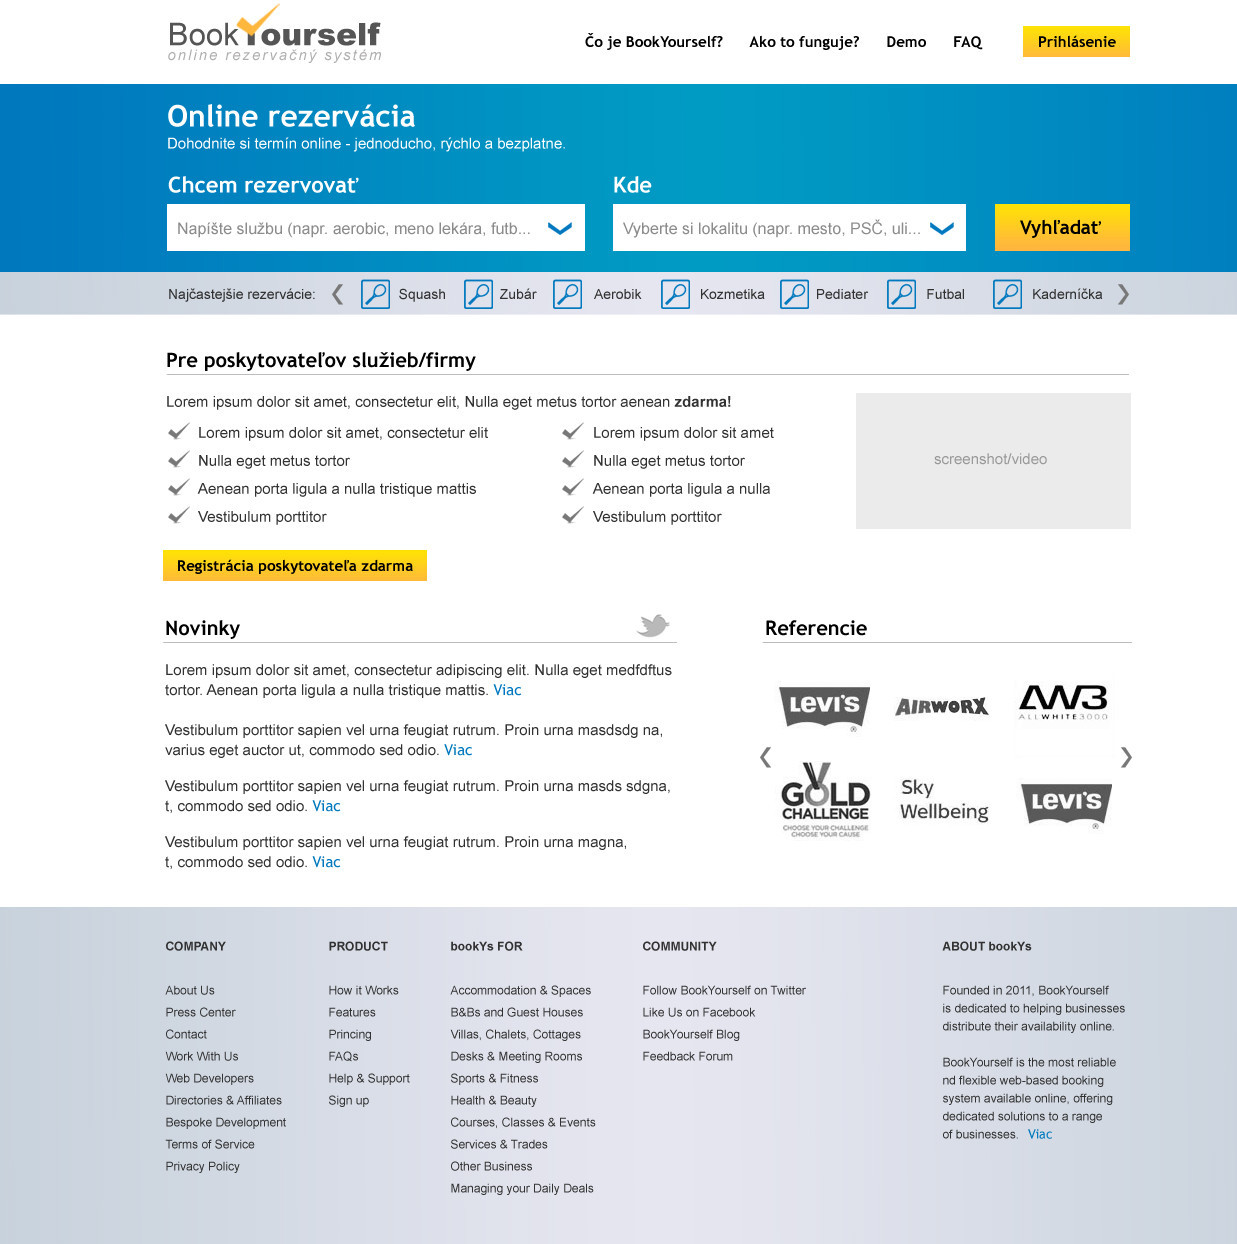
\includegraphics[scale=0.25]{images/homepage.jpg} % sem dajte cestu k obrazku, scale nastavuje, ako je to velke :)
		\caption{Domovská stránka}                        % popis pod obrazkom, treba ho dat, nech sa potom zobrazuje aj v zozname ilustracii
		\label{img:homepage}                              % a znova label, pre zmenu pouzijeme img: aby bolo jasne, ze je to obrazok a potom nejaky slug
\end{figure}

A este citacia, takze jednoducho pouzijeme prvu vec z bibliografickeho zaznamu na odkazanie na neho a citaciu pridame jednoducho takto
\cite{alertbox}
